\documentclass[11pt, oneside]{article}   	% use "amsart" instead of "article" for AMSLaTeX format
\usepackage{geometry}                		% See geometry.pdf to learn the layout options. There are lots.
\geometry{letterpaper}                   		% ... or a4paper or a5paper or ... 
%\geometry{landscape}                		% Activate for for rotated page geometry
%\usepackage[parfill]{parskip}    		% Activate to begin paragraphs with an empty line rather than an indent
\usepackage{graphicx}				% Use pdf, png, jpg, or eps� with pdflatex; use eps in DVI mode
								% TeX will automatically convert eps --> pdf in pdflatex	
\graphicspath{{figures/}} 				% Location of the graphics files	
\usepackage{amssymb}
\usepackage{xcolor}


\begin{document}
%\pagestyle{empty}


\begin{center}
\bf \LARGE
P3MD LAB -\\PROBE STATION INSTRUCTIONS v2.2
\end{center}
\vspace{5mm}

The semi-automatic probe station, Cascade Summit 12000 series, is located in the P3MD Lab in Physics-360. This document describes the various parts of  the probe station, and describes instructions on using the probe station. Please follow the instructions below in order to use the probe station.


%Section 1 - Entering the soft-wall clean room with proper attire
\section{Entering the soft-wall clean room with proper attire}
Entering the clean room without proper attire is strictly prohibited. Figure 1 shows a cap, face mask, lab coat, gloves and shoe covera which need to be worn before entering the clean room. Also, wearing anti-static devices and testing them before entering clean room is recommended. Always make sure that you are in proper attire before you enter the clean room.

\begin{figure}[h!]
	\centering
	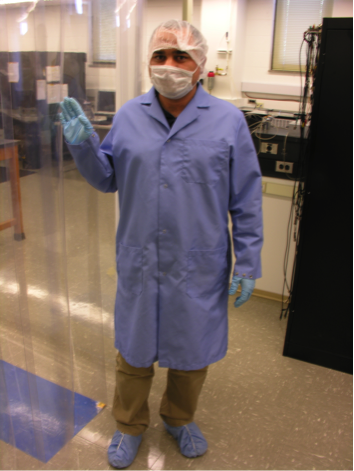
\includegraphics[width=0.5\textwidth]{attire.png}
	\caption{Proper clean room attire.}
\end{figure}


%Section 2 - Observe the probe station hardware
\section{Observe the probe station hardware}
Figure 2 shows the major components of Probe Station unit. The unit consists of:
\begin{enumerate}
\begin{enumerate}
	\item The Cascade Summit probe station
	\item Keithley instruments (237 Source meter, K6485 Ammeters)
	\item LCR meter (for CV measurements)
	\item Switching matrix
	\item Temptronic chiller
	\item Cables
	\item Vacuum holder (Linicon)
	\item A-Zoom focus and light switch
\end{enumerate}
\end{enumerate}

\begin{figure}[h!]
	\centering
	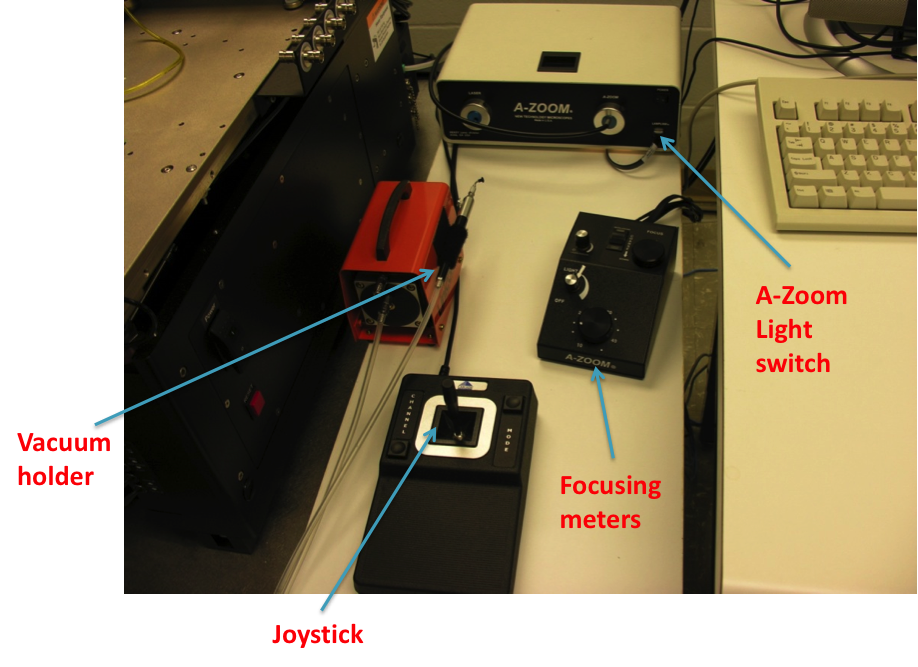
\includegraphics[width=\textwidth]{instruments.png}
	\caption{Light switch, Vacuum wafer holder, Joystick, and Focusing dial.}
\end{figure}

The probe station will be used for measuring IV and CV of the different pad positions on a wafer. The K6485 are Picoammeters or Picometers used for measuring currents from pads on the wafer. Th Keithley 237 Source meter is used to supply bias to the wafer using chuck bias. The LCR meter is used for low frequency as well as high frequency CV measurements (limit is -500V). The switching matrix is used to switch between IV and CV measurements directly, without changing the setup (not yet used for the current setup). The Temptronic thermal system is used to maintain the wafer at a given temperature.

Figure 2 shows the various instruments used for focusing and holding the wafer. The A-Zoom box provides the light for viewing the wafer during setup and needs to be switched off manually when the measurements are made. A-Zoom also provides focusing using two meter dials as shown. Figure 2 also shows the joystick which can be used for moving the focus to various positions on the wafer. The vacuum wafer holder is also shown in Figure 2. The vacuum holder only works when the switch on its side is pressed on. Letting go of the switch turns off the vacuum and wafer will fall down, SO PLEASE MAKE SURE TO KEEP PRESSING THE SWITCH ON WHILE USING THE VACUUM HOLDER. 

\vspace{2mm}
{\color{red}
IF YOU SEE ANY INSTRUMENT NOT WORKING OR NOTICE ANYTHING UNUSUAL, PLEASE INFORM A SENIOR IN THE LAB IMMEDIATELY!}
\vspace{2mm}

\begin{figure}[h!]
	\centering
	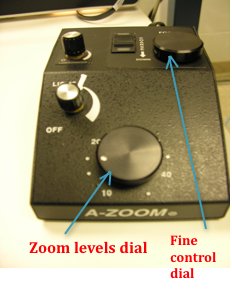
\includegraphics[width=0.37\textwidth]{zoom_controls.png}
	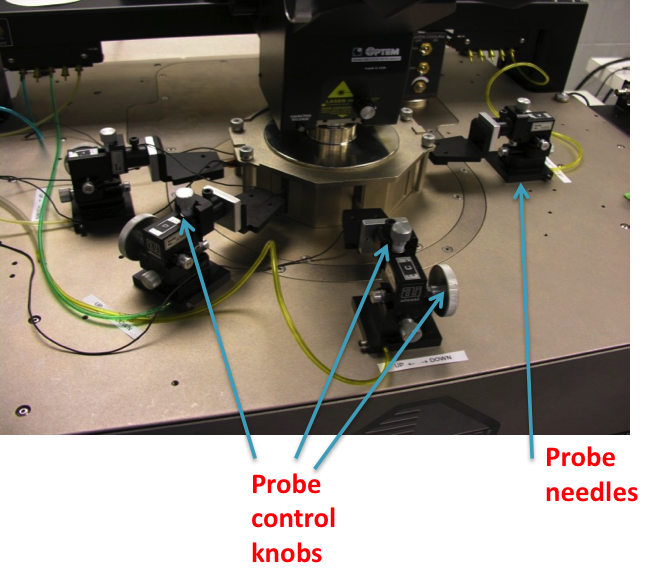
\includegraphics[width=0.53\textwidth]{probe_needles.png}
	\caption{Zoom controls and Probe needles.}
\end{figure}

Figure 3 shows the focusing dials of A-Zoom in more detail. There are two knobs for coarse and fine-grained control. There is also a light switch for switching the light inside the chamber. Also, notice the different zoom levels on dial (10, 20, etc.). The zoom level will be important when the probe positions are defined later.

Figure 3 also shows the four probe needles. There are controls for moving the probe needles left-right, up-down and, most importantly, lower-higher. The left-right and up-down knobs move the probe needle in XY plane. The lower-higher (in Z direction) moves the probe needles towards or away from the wafer. When the needles are away from wafer, they appear as 2 needles, while when the needles are close to wafer, they appear as single needles. All the needle control knobs are very sensitive and should be used slowly and carefully. 


%Section 3 - Probes and cabling
\section{Probes and cabling}
The output of K237 provides the bias to the chuck, which goes to the probe station. Also, the outputs from probes are connected to Pins 1 and 2 on the top of the probe station. These outputs are connected by BNC connectors to the Keithley 6485 picometers. All the COM terminals of 6485 and 237 are connected together to form a common ground. All units are also connected to a PC using GPIB cables. These different GPIB cables are daisy-chained together and all the bias voltages and current measurements can be displayed and recorded on the computer using GPIB connections. LabView code is used to measure both IV and CV data and automatically apply bias using the display panel on the computer.

The IV measurement is done first over all pad positions defined in the wafer map. After the IV measurement is done, CV measurements are taken. The LCR meter must be manually connected as in Figures 4 and 5. Output Hi and Output Lo pins of K237 are connected to red and black input pins at the back of the LCR meter as shown in Figure 5. Also, the RED pins at the front of the LCR meter are connected to the Chuck bias at the back of the probe chamber (similar to how the K237 was connected for the IV test). The black pin at the front of the LCR meter receives the measured capacitance value from the probe needle and is connected back to the LCR meter via Pin 1.

\begin{figure}[h!]
	\centering
	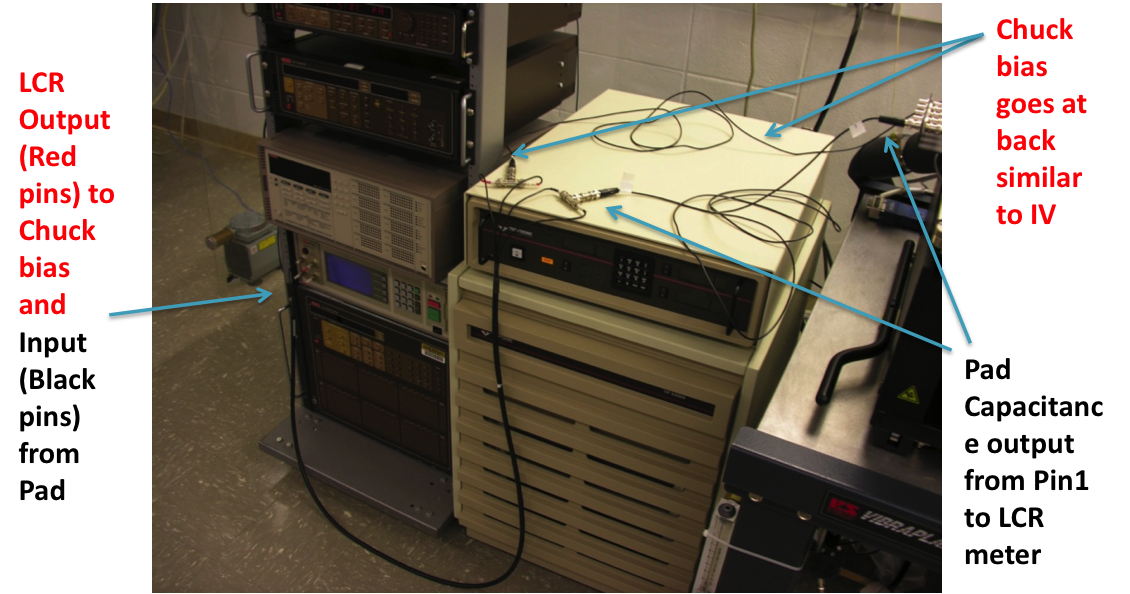
\includegraphics[width=0.9\textwidth]{outputs1.png}
	\caption{Outputs from LCR meter to bias and Probe Station to LCR meter.}
\end{figure}

\begin{figure}[h!]
	\centering
	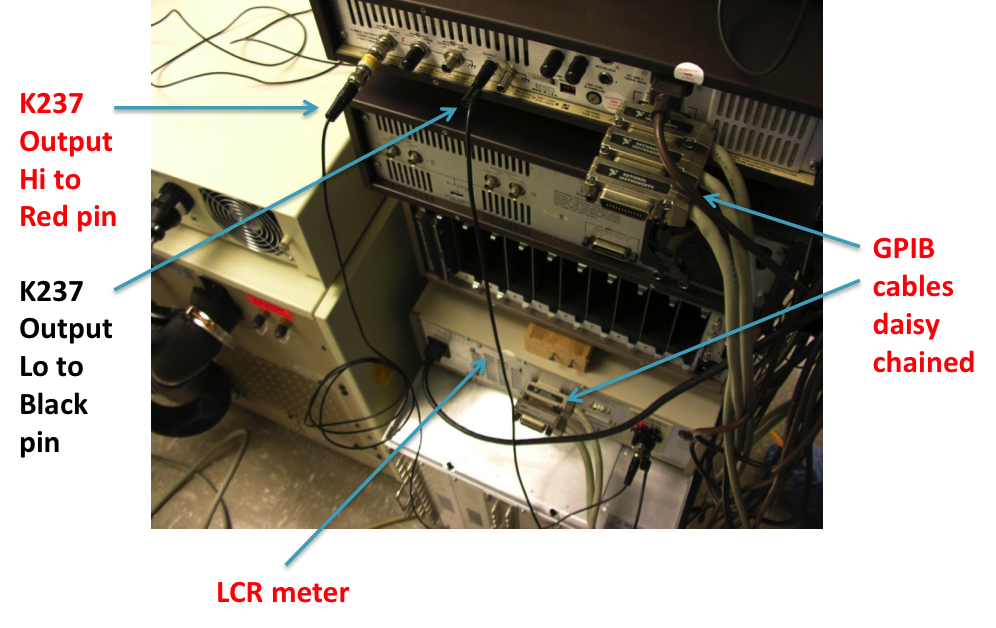
\includegraphics[width=0.9\textwidth]{outputs2.png}
	\caption{Outputs from K237 and LCR meter to Probe Station.}
\end{figure}

\newpage
\vspace{2mm}
{\color{red} \centering \large
NOW YOU ARE READY TO SET UP THE SOFTWARE!}
\vspace{2mm}


%Section 4 - Run "Nucleus" on PC's desktop
\section{Run Nucleus on PC's desktop}
Open Nucleus by double-clicking the Nucleus icon 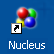
\includegraphics[width=.05\textwidth]{nucleus_icon.png} on the desktop. The login credentials are as follows:

\hspace{7mm}Login name: Superuser

\hspace{7mm}Password: cascade

The main windows that open are the Nucleus main panel, Live Video, and Motion Control.

\begin{enumerate}
\begin{enumerate}
	\item First, click the {\it ``Wafer Load''} button 
\includegraphics[width=.05\textwidth]{wafer_load.png} in the motion control sub-window. The Live Video window will show the focus position moving from the center of the chuck to the top edge of the chuck.
	\item Next, open the probe station micro-chamber door. A message will be displayed saying that the wafer access interlock is open. The chuck and chuck interlock should be visible as shown in Figure 6. Unlatch the chuck interlock and pull out the chuck. Pull the chuck all the way back until you feel a click. The chuck should now be held in place and will not go back after you let go of the latch.
	\item Check to make sure that the {\it ``Vacuum Off''} button 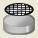
\includegraphics[width=.05\textwidth]{vacuum_off.png} in the main panel is set, indicating that the chuck's vacuum is off. Otherwise, the vacuum will be ON before you place the wafer down.
	\item Check to make sure the chuck surface and conductive rubber (if being used) are both clean. If the surfaces are dirty, clean them using IPA solution.
\end{enumerate}
\end{enumerate}

\begin{figure}[h!]
	\centering
	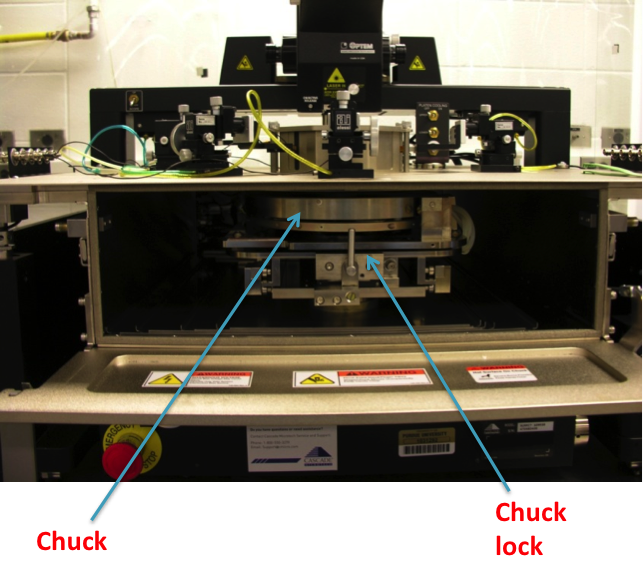
\includegraphics[width=0.455\textwidth]{chuck1.png}
	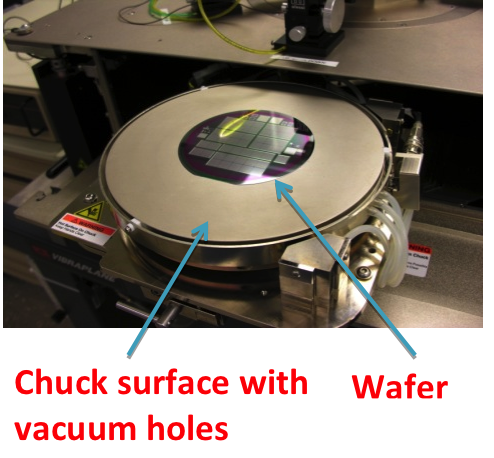
\includegraphics[width=0.445\textwidth]{chuck2.png}
	\caption{Chuck and loading surface.}
\end{figure}

%Section 5 - Wafer loading
\section{Wafer loading}
\begin{enumerate}
\begin{enumerate}
	\item Check if the lever arm is down. If not, lower the lever arm.
	\item Make sure the vacuum pump is turned on.
	\item Take a wafer from the dry box cabinet in the soft-wall clean room. Use the vacuum holder to lift the wafer from the wafer box. Use tweezers or spatula-like pinchers to hold the end of wafer while vacuum holder is still on. Be very careful when handling the wafer.
	\\{\color{red}IMPORTANT: Make sure that the vacuum holder black button is always PRESSED ON when the wafer is held; otherwise the wafer will fall on ground.}
	\item Put the wafer slowly in the center of the conductive rubber. Once the wafer is placed on the chuck, release the vacuum button to leave the wafer on the chuck.
	\\{\color{red}IMPORTANT: Once the wafer is released from the vacuum pen it may slide around on the rubber.}
	\item Check that the wafer has been placed in the center of the chuck and make sure that all the vacuum holes on the conductive rubber are covered. If the wafer is not centered, move it slowly to the center. Make sure you always handle the wafer along the flat edge. Also, note that the flat edge must be facing you when you place it.
	\item Press the {\it ``Vacuum On''} button in the main panel (same location as the {\it ``Vacuum Off"} button, should look like this when the vacuum is on: 
\includegraphics[width=.05\textwidth]{vacuum_on.png}). Check with the tweezer or vacuum pen that the wafer is stuck to chuck and does not move.
	\item Align the wafer as much as possible using an eyeball estimate. To do this, use the latch to push the wafer towards the micro-chamber so that edge of micro-chamber door is parallel to any of the major lines on the wafer. If the wafer is not aligned, turn off the vacuum and very slowly move the wafer to align it to edge of the chamber. Try to align it as much as possible. Fine alignment of the wafer will be done using software.
	\item If the vacuum is off, turn it back on in the Nucleus window.
	\item Push the chuck back into the probe station chamber and lock the latch.
	\item Close the micro-chamber gate.
	\item Turn the light ON by flipping the A-Zoom power switch.
	\item In Nucleus click the {\it ``Wafer Center''} button 
\includegraphics[width=.05\textwidth]{wafer_center.png} in the motion control window.
\end{enumerate}
\end{enumerate}


\newpage
%Section 6 - Wafer alignment
\section{Wafer alignment}
{\color{red} If simply performing an IV test on a module or single-chip sensor, skip this section as well as the next and proceed to section 8: Probe tip setup.}
\begin{enumerate}
\begin{enumerate}
	\item Zoom in (\textless 30) and adjust the focus.
	\item Click on the tools tab in the Nucleus window and select {\it Align} and make sure the following options are set:
	\begin{enumerate}
		\item {\it Start at center}: OFF
		\item {\it Scan velocity}: Fast
		\item {\it Scan method}: Wait at end
		\item {\it Scan distance}: Define with Joystick
	\end{enumerate}
	\item Click {\it ``Start Align''}. The Align procedure scans back and forth between two fixed points, stopping at each end point and asking if the alignment should continue.
	\begin{enumerate}
		\item Select the LEFT end point.
		\item Select the RIGHT end point.
		\item When selecting end points, make sure they both lie along the same visible line on the wafer. Pick a horizontal that is as long as possible.
	\end{enumerate}
	\item Click {\it ``Continue''} and the procedure will travel from one end point to the other. You should notice that after it reaches the second endpoint it will have deviated by some angle from the wafer line.
	\item At the second endpoint, note the deviation from the wafer line and adjust the theta knob until the crosshair is half the deviated angle from the wafer line. Then click {\it ``Continue''}.
	\item The Alignment procedure should move back to the 1st endpoint. Once there move the crosshair back to the wafer line that you are using for alignment and then hit {\it ``Continue''}. NOTE: Do NOT adjust the theta knob at the 1st endpoint to align the crosshair, only move using the Nucleus controls to adjust the crosshair position.
	\item Repeat steps e-f until the crosshair stays parallel with the wafer line, that is there is no visible deviation as the crosshair travels from one endpoint to the other.
	\item Click {\it ``No''} when it asks to continue and then {\it ``Close''}. The wafer should now be officially aligned
\end{enumerate}
\end{enumerate}


\newpage
%Section 7 - Setting up the wafer map
\section{Setting up the wafer map}
\begin{enumerate}
\begin{enumerate}
	\item First move the crosshair to Site 1 on the wafer. For the 6-inch wafers this is the diode in the lower left corner as shown in Figure 7.
	\item Align the crosshair over the top left contact pad. Make sure that the probe tips can reach their respective pads.
	\item If not already open, open the Wafer Map window from the Nucleus window.
	\item Make sure that the correct wafer map is loaded. To check this, simply look at the top of the Wafer Map window and note the name of the wafer map. For the 6-inch wafers the correct wafer map is ``2013\_6-inch\_wafer\_map1.wfd''.
	\item Right click on the Live Video window and select {\it ``Set Reference in Place''}.
	\item Click on the {\it ``Sub Die''} button in the Wafer Map window. This will open another window that shows the relative positions of all the sites with respect to Site 1. If the reference position was correctly set to Site 1, double clicking on any of the other site numbers in the Sub Die window will move the probes to that site. If, after selecting another site, the probes do not move to the correct location, either the wrong wafer map is loaded or the reference position was not set correctly.
	\vspace{1mm}
	\\NOTE: In Nucleus, the site numbers are counted starting from 0, so Site 1 in Nucleus is Label 0, Site 21 is Label 20, and so on.
\end{enumerate}
\end{enumerate}

\begin{figure}[h!]
	\centering
	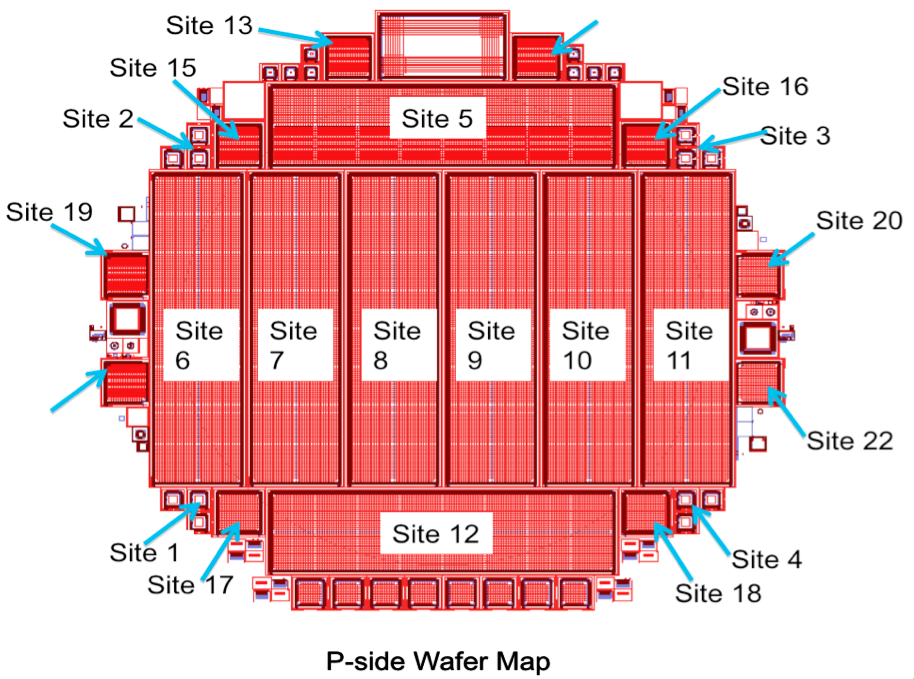
\includegraphics[width=0.7\textwidth]{wafer.png}
	\caption{Site layout for 6-inch wafer.}
\end{figure}


%Section 8 - Probe tip setup
\section{Probe tip setup}
We are now ready to start the IV/CV scan. Make sure the Keithleys are connected properly to the probe tips and chuck.
\begin{enumerate}
\begin{enumerate}
	\item Before moving to contact, check the contact settings. Right-click the {\it ``Move Z Stage to Contact''} button 
\includegraphics[width=.05\textwidth]{z_stage_contact_off.png} and ensure that the settings under ``Chuck'' are as follows:
	\begin{enumerate}
		\item {\it Contact}: 1000 um
		\item {\it Separate Distance}: 500 um
	\end{enumerate}
	\item Make sure ALL of the probes are a safe Z-distance above the wafer, then click on the {\it ``Move Z Stage to Contact''} button 
\includegraphics[width=.05\textwidth]{z_stage_contact_off.png}. The symbol should turn green 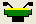
\includegraphics[width=.05\textwidth]{z_stage_contact_on.png}, indicating that the probe station is in contact mode. While in this mode you cannot move the chuck using the Nucleus software.
	\item Move the probes above their respective pads. The probe tip that comes in at an angle is usually used for the Active area and the other probe tip is used for the Guard-ring.
	\vspace{1mm}
	\\NOTE: Make sure that the wires connecting the probe tips to the K6485s are correctly labeled, the K6485 with GPIB address 10 is used for measuring the Guard-ring and the K6485 with GPIB address 14 is used for measuring the Active area.
	\item Using the knobs on the probe station, lower the probe tips into contact with the pads. If the K6485s are in local mode you should hear a set of clicks when the probe tips first make contact with the pads and the K6485s should also be reading small current value. You should also see the probe tips move forward slightly when they make contact.
	\item Turn the light off.
\end{enumerate}
\end{enumerate}


\newpage
%Section 9 - IV/CV measurement
\section{IV/CV measurement}
\begin{enumerate}
\begin{enumerate}
	\item Open ``C:\textbackslash Documents and Settings\textbackslash PROBER\textbackslash My Documents\textbackslash GitHub\textbackslash probestation\textbackslash\\Automatic\_IV\_CV\_with\_XML\_Global\_Stop\_V1.2.vi''.\\{\color{red}(For a simple IV scan of a module or single chip sensor, instead open\\``Manual IV\_K237\_K6485\_V1.4 with XML Output.vi" and skip any steps in this process that are blue. That should give you a rough guideline of your process.)}
	\item On the front panel, set values for voltage ranges and voltage step size for both the IV and CV scans. {\color{blue}Also, make sure the site number is set to the appropriate values for the IV and CV scans (for the 6-inch wafer there should be 22 sites for the IV scan and 12 for the CV scan).} Finally make sure the file path is set to an appropriate location as this is where the data will be saved.
	\item Run the program.
	\item You will be prompted to fill out various fields that are used to document the data:
	\begin{enumerate}
		\item {\it Wafer ID\#}: The ID number of the wafer currently being tested.
		\item {\it Name of Test}: This will create a folder with the specified name which will be the location for all the data collected for that particular run. If a folder with the name already exists, then a second folder will be created with an appended number. This ensures that each folder contains only one set of data.
		\item {\it Comment Description} (optional): A field used in the XML output.
		\item {\it User} (optional): A field used in the XML output
	\end{enumerate}
	{\color{blue}\item Next a prompt to Skip Subsite will appear, if for whatever reason you do not wish to collect data on this site click {\it ``Skip''}, otherwise click {\it ``Continue''}.}
	\item At this point the Labview code makes a check to see if the probe tips are in contact. If they are not, an error window will appear indicating that the probes did not go into contact with the pads. If the error occurs, follow these steps:
	\begin{enumerate}
		\item Check to make sure that the K237 is in Standby mode. If it isn�t, attempt to manually set it to standby mode.
		\item Turn on the light.
		\vspace{1mm}
		\\NOTE: If the K237 is not in Standby mode when the light is switched on you WILL arc the sensor and possibly ruin the entire wafer. So make sure that the light is only turned on when the K237 is in standby.
		\item Check to see if the probes are still aligned with their respective pads. If they are, very gently lower the probe tips until they are in contact with the pads.
		\item Another possibility for the contact check is that the probe station did not go back into contact mode after moving to the site. To check this, look at the status of the Stage Height in the Motion Control window. If it is set to {\it ``Separate''} 
\includegraphics[width=.05\textwidth]{z_stage_separate_on.png} check to make sure the probes are aligned above their respective pads and then click {\it ``Move Z Stage to Contact''} 
\includegraphics[width=.05\textwidth]{z_stage_contact_off.png}.
		\item VERY IMPORTANT: Turn the light off.
		\item Retry the contact check. If the error occurs again, repeat steps i-v or choose to skip the current site.
		\vspace{1mm}
		\\NOTE: If the contact check failed due to the stage being stuck in Separate mode, the stage will remain in Separate mode for the remainder of the scan unless you move it back to Contact mode. Make sure you only do this during the contact check error window and make sure that the probes are in the correct positions before changing the stage mode.
	\end{enumerate}
	\item When the contact check passes, the Labview code will begin the IV scan and data should begin to appear on the graphs in the Front Panel.
	{\color{blue}\item After the scan completes for the current site the code will move to the next site, so repeat steps e-g.
	\item After all the sites have been scanned, a new window will appear indicating that the IV scan is complete. At this point switch the wiring setup to CV by following the substeps below. Only after you are sure that the wiring is correct should you hit continue.
	\begin{enumerate}
		\item Take the cable for the bias from the back of the Kiethley and plug it into the red T-junction input.
		\item Take the cable for the active area from the GPIB14 meter and plug it into the black T-junction input.
		\item Connect the back of the LCR meter to the source meter, using the wire that is hanging on the rack at the side. Here, you should be connecting the Kiethley to the QuadTech.
	\end{enumerate}
	\item A similar window asking if you would like to skip the current subsite will appear during the CV scan. Click {\it ``Skip''} if you do not wish to take data for the current site or {\it ``Continue''} if you do.}
\end{enumerate}
\end{enumerate}


\newpage
%Section 10 - Shutting down
\section{Shutting down}
\begin{enumerate}
\begin{enumerate}
	\item Make sure that all the instruments are in Standby and sourcing no voltage.
	\item Turn the light ON.
	\item Manually raise the probe tips well above the wafer using the knobs on the probe station.
	\item Click the {\it ``Move the Z Stage to separate''} button 
\includegraphics[width=.05\textwidth]{z_stage_separate_off.png} in the Motion Control window. It should turn red to indicate that the probe station is in separate mode 
\includegraphics[width=.05\textwidth]{z_stage_separate_on.png}.
	\item Click the {\it ``Wafer Load''} button 
\includegraphics[width=.05\textwidth]{wafer_load.png} the Nucleus Motion Control window. This will bring the chuck forward so that it can be pulled out and accessed easily.
	\item Open the micro-chamber gate. Pull out the chuck and secure it in place.
	\item Click the {\it ``Turn Vacuum OFF''} symbol (should look like this when the vacuum is turned off: 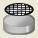
\includegraphics[width=.05\textwidth]{vacuum_off.png}) on the Nucleus window.
	\item Use the Vacuum Pen and spatula to very carefully remove the wafer from the conductive rubber. This step can take a very long time and it is very important that the wafer is removed carefully as the rubber will have adhered to the wafer, making peeling the wafer off of the rubber very tricky.
	\item Place the wafer back in its case. Make sure that you place it in the correct side of the wafer container.
	\item Place the wafer container back in the dry box.
	\item Return the chuck and close the micro-chamber gate.
	\item Turn the light OFF.
\end{enumerate}
\end{enumerate}


%\vspace{10mm}
%This concludes the tutorial for operating the probe station for an Automatic IV/CV scan.


\end{document}
